

%-------Introduction-----------------------------------------------------------


\begin{frame}{Introduction}{The System}
  \begin{figure}[H]
    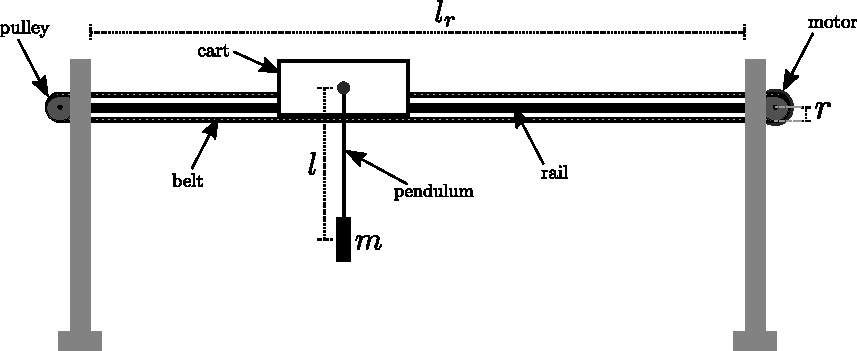
\includegraphics[width=1\textwidth]{figures/systemSetup}
  \end{figure}
\end{frame}

\begin{frame}{Introduction}{Task}
  \begin{figure}[H]
    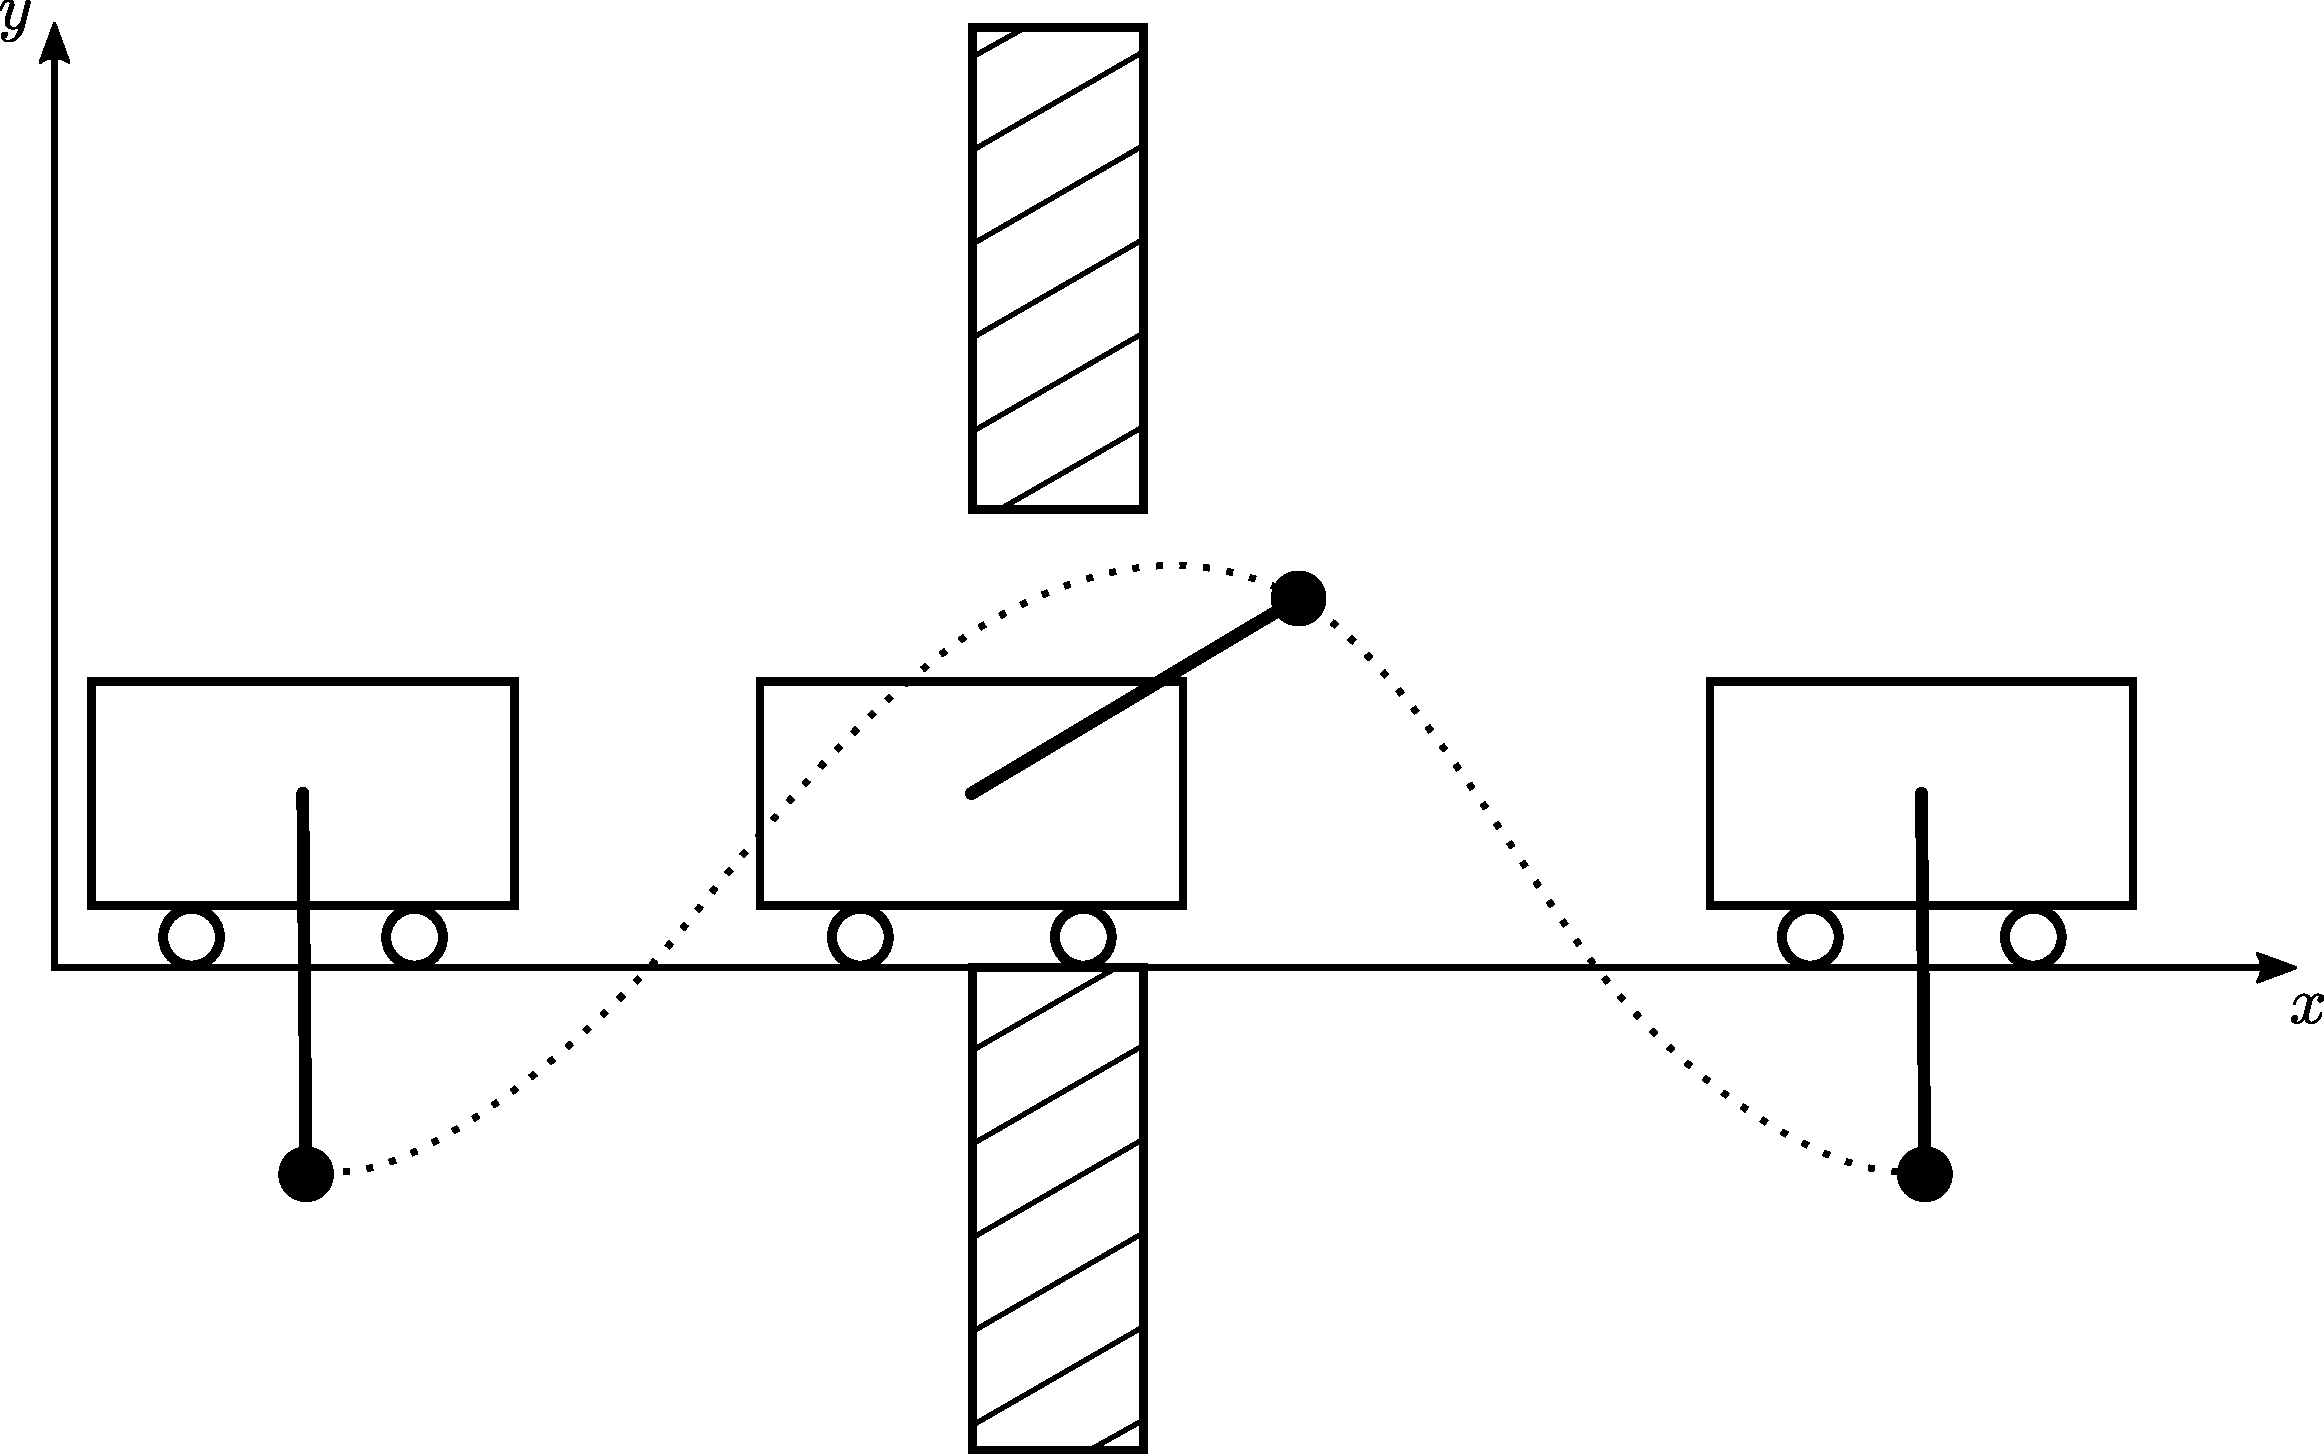
\includegraphics[width=.85\textwidth]{figures/systemTask}
  \end{figure}
\end{frame}


%-------Modelling-----------------------------------------------------------


\begin{frame}{Modeling}{Conventions and Assumptions}
  \small
  \vspace{-1cm}
  \begin{figure}[H]
    \begin{minipage}{0.45\linewidth}
      \begin{figure}[H]
        \hspace{-3cm}
        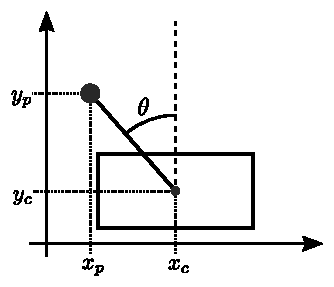
\includegraphics[width=1\linewidth]{figures/excessiveCoordinates}
      \end{figure}        
    \end{minipage}\hspace{-1cm}
    \begin{minipage}{0.45\linewidth}
      \begin{figure}[H]
        \vspace{.2cm}
        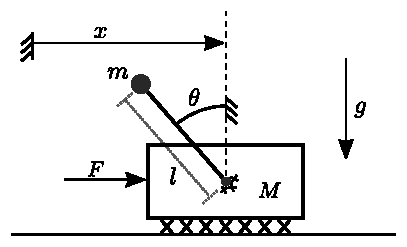
\includegraphics[width=1.3\linewidth]{figures/mechanicalDrawing}
      \end{figure}\hspace{1cm}
    \end{minipage}
  \end{figure}
  \vspace{-.3cm}
  \begin{flalign}
    \hspace{-10pt}
    \begin{cases}
      x_c &=  x  \\
      y_c &=  0  
    \end{cases} & \nonumber
    \hspace{5pt}
    \begin{cases}
      x_p &=  x - l\sin \theta \\
      y_p &=  l\cos \theta
    \end{cases} & \nonumber
    \hspace{-4pt}
    \begin{cases}
      \dot{x}_p &= \dot{x} - l\cos \theta \dot{\theta} \\
      \dot{y}_p &= -l\sin \theta \dot{\theta}
    \end{cases} &\nonumber
    \hspace{5pt}
    \begin{cases}
      \ddot{x}_p = \ddot{x} + l \sin \theta \dot{\theta}^2 - l\cos \theta \ddot{\theta} \\
      \ddot{y}_p = -l\cos \theta \dot{\theta}^2  -l\sin \theta \ddot{\theta}
    \end{cases}  & \nonumber
  \end{flalign}
  \normalsize
\end{frame}

\begin{frame}{Modeling}{Newton's Method}
  \small
  \begin{figure}[H]
    \vspace{-1cm}\hspace{.1cm}
    \begin{minipage}{0.45\linewidth}
      \begin{figure}[H]
        \hspace{-2cm}
        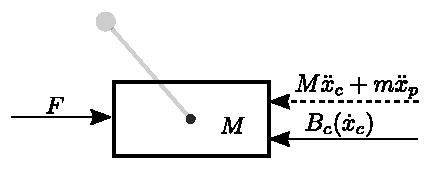
\includegraphics[width=1.2\linewidth]{figures/freeBodyCart}
      \end{figure}        
    \end{minipage}\hspace{-1cm}
    \begin{minipage}{0.45\linewidth}
      \begin{figure}[H]
        \vspace{-.25cm}
        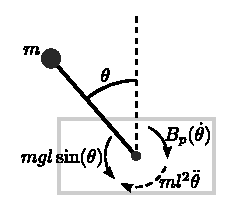
\includegraphics[width=.8\linewidth]{figures/freeBodyPendulum}
      \end{figure}\hspace{1cm}
    \end{minipage}
  \end{figure}
  %
  \begin{minipage}{0.45\linewidth}
    \vspace{-1.3cm}
    \begin{flalign} \hspace{.1cm}
      M\ddot{x}_c + m\ddot{x}_p &= F - B_c(\dot{x}_c) & \nonumber
    \end{flalign}
  \end{minipage}
  \begin{minipage}{0.45\linewidth}
    \vspace{-1.5cm}
    \begin{flalign} \hspace{7cm}
      ml^2 \ddot{\theta} &= mgl \sin \theta - B_p(\dot{\theta}) & \nonumber \\
      - ml\ddot{x}_p \cos \theta - ml\ddot{y}_p \sin \theta &=  mgl \sin \theta - B_p(\dot{\theta}) & \nonumber
    \end{flalign}
  \end{minipage}

  \begin{flalign}
    \begin{cases}
      ml^2 \ddot{\theta} - ml\cos \theta \ddot{x} - mgl \sin \theta &= - B_p(\dot{\theta}) \\
      ( M + m ) \ddot{x} + ml\sin \theta \dot{\theta}^2 - ml\cos \theta \ddot{\theta} &= F - B_c(\dot{x}) 
    \end{cases} & \nonumber
  \end{flalign}
  \normalsize
\end{frame}


\begin{frame}{Modeling}{Energy Method}
  \small
  \begin{minipage}{0.45\linewidth}
    \vspace{-.3cm}
    \begin{flalign} \hspace{.1cm}
      U &= mg\overbrace{l( 1 + \cos \theta )}^{h} + 0  \nonumber  &  \\
      T &= \tfrac{1}{2} m \dot{x}_p^2 + \tfrac{1}{2} m \dot{y}_p^2  + \tfrac{1}{2} M \dot{x}_c^2 \nonumber & 
    \end{flalign}
  \end{minipage}
  \begin{minipage}{0.45\linewidth}
    \vspace{-1.5cm}
    \begin{flalign}\hspace{5cm}
      U &= mgl( 1 + \cos \theta )   & \nonumber  \\
      T &= \frac{1}{2} ( M + m ) \dot{x}^2 - m \dot{x} l \cos \theta \dot{\theta} + \frac{1}{2} m l^2 \dot{\theta}^2 & \nonumber
    \end{flalign}
  \end{minipage}
  \begin{flalign}
    \cal{L} &= T - U & \nonumber \\ 
    \cal{L} &= \tfrac{1}{2} ( M + m ) \dot{x}^2 - m \dot{x} l \cos \theta \dot{\theta} + \tfrac{1}{2} m l^2 \dot{\theta}^2 - m g l( 1 + \cos \theta ) &  \nonumber
  \end{flalign}
  \begin{flalign}
    \frac{d}{dt}  \frac{\partial \cal{L}}{\partial \dot{\vec{q}}} - \frac{\partial \cal{L}}{\partial \vec{q}}  &=  \vec{Q}  && \nonumber
  \end{flalign}
  \begin{flalign}
    \begin{cases}
      ml^2 \ddot{\theta} - ml\cos \theta \ddot{x} - mgl \sin \theta &= - B_p(\dot{\theta}) \\
      ( M + m ) \ddot{x} + ml\sin \theta \dot{\theta}^2 - ml\cos \theta \ddot{\theta} &= F - B_c(\dot{x}) 
    \end{cases} && \nonumber
  \end{flalign}
  \normalsize
\end{frame}

\begin{frame}{Modeling}{Friction Model}
  \small
  \vspace{-1cm}
  \begin{figure}[H]\hspace{-3cm}
    \begin{minipage}{0.3\linewidth}
      \begin{figure}[H]
        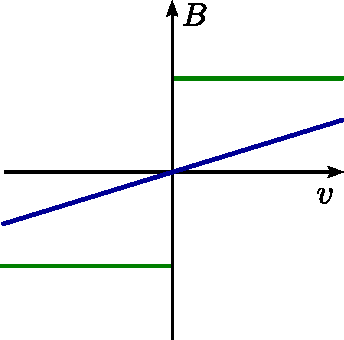
\includegraphics[width=.8\linewidth]{figures/coulombViscous1}
      \end{figure}        
    \end{minipage}%\hspace{-1cm}
    \begin{minipage}{0.3\linewidth}
      \begin{figure}[H]
        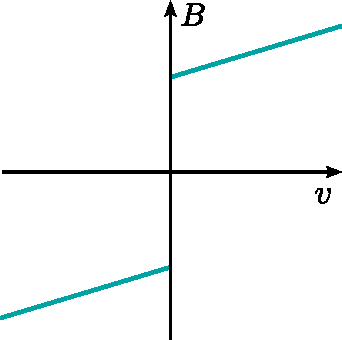
\includegraphics[width=.8\linewidth]{figures/coulombViscous2}
      \end{figure}
    \end{minipage}%\hspace{-1cm}
    \begin{minipage}{0.3\linewidth}
      \begin{figure}[H]
        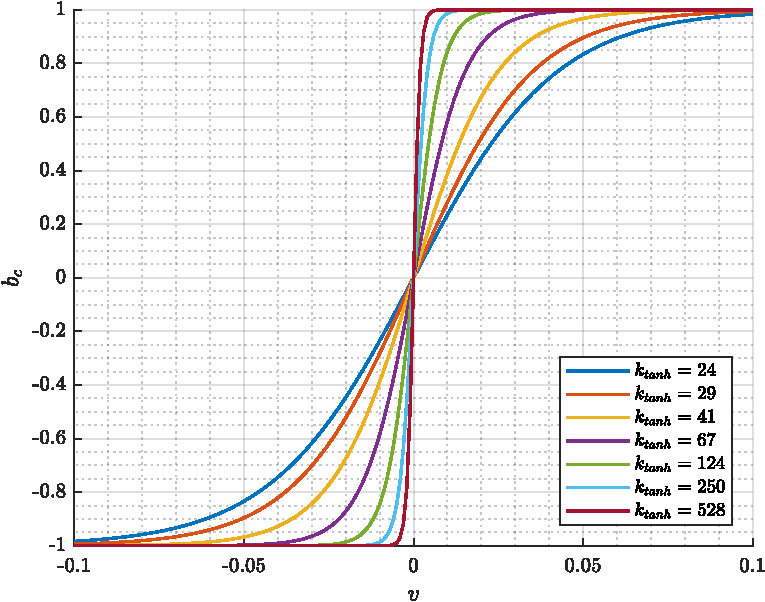
\includegraphics[width=1.7\linewidth]{figures/tanhApprox}
      \end{figure}
    \end{minipage}
  \end{figure}
  \vspace{-.2cm}
  \begin{minipage}{0.3\linewidth}
    \begin{flalign}
      B_p(\dot{\theta}) &= b_{p,v} \dot{\theta} + \text{sgn}(\dot{\theta}) b_{p,c} & \nonumber \\
      B_c(\dot{x})      &= b_{c,v} \dot{x}      + \text{sgn}(\dot{x}) b_{c,c} & \nonumber
    \end{flalign}
  \end{minipage}\hspace{1.7cm}
  \begin{minipage}{0.3\linewidth}
    \begin{flalign}
      B_p(\dot{\theta}) &= b_{p,v} \dot{\theta} + \tanh(\text{k}_\text{tanh}\dot{\theta}) b_{p,c}  & \nonumber \\
      B_c(\dot{x})      &= b_{c,v} \dot{x}      + \tanh(\text{k}_\text{tanh}\dot{x}) b_{c,c}   &  \nonumber
    \end{flalign}
  \end{minipage}
  \normalsize
\end{frame}


%-------Nonlinear Control--(System Transformation)-----------------------------


\begin{frame}{Nonlinear Control}{System Transformation}
\small
\vspace{-.5cm}
%\begin{flalign}
%\dot{\vec{\eta}} &=  f_a(\vec{\eta},\vec{\xi}) \nonumber  \\
%\dot{\vec{\xi}}  &=  f_b(\vec{\eta},\vec{\xi}) + g_b(\vec{\eta},\vec{\xi}) F  & \nonumber
%\end{flalign}
\begin{flalign}
\begin{bmatrix}
m l^2              & -m l \cos \theta  \\
-m l \cos \theta   & M + m
\end{bmatrix}
\begin{bmatrix}
\ddot{\theta}  \\
\ddot{x}
\end{bmatrix}
+
\begin{bmatrix}
0  \\
m l \sin \theta \dot{\theta}^2
\end{bmatrix}
+
\begin{bmatrix}
B_p(\dot{\theta})  \\
B_c(\dot{x})
\end{bmatrix}
+
\begin{bmatrix}
-m g l \sin \theta  \\
0
\end{bmatrix}
&=
\begin{bmatrix}
0  \\
F
\end{bmatrix}  & \nonumber
\end{flalign}
%
\vspace{.5cm}
\begin{minipage}{1\linewidth}\hspace{7cm}
  $[\ x_1\ x_2\ x_3\ x_4\ ]^T = [\ \theta\ x\ \dot{\theta}\ \dot{x}\ ]^T $
\end{minipage}
%
\vspace{-1.2cm}
\begin{flalign}
&\vec{M}(\vec{q})\ddot{\vec{q}} + \vec{C}(\vec{q},\dot{\vec{q}}) + \vec{B}(\dot{\vec{q}}) + \vec{G}(\vec{q}) = \vec{F}  & \nonumber \\
&\ddot{\vec{q}}
=
\vec{M}^{-1}(\vec{q})
\left(
\vec{F} -\vec{C}(\vec{q},\dot{\vec{q}}) -\vec{B}(\dot{\vec{q}}) -\vec{G}(\vec{q})
\right)  \nonumber &
\end{flalign}
%
\begin{flalign}
\begin{bmatrix}
\dot{x_1} \\
\dot{x_2} \\
\dot{x_3} \\
\dot{x_4}
\end{bmatrix}
&=
\begin{bmatrix}
x_3  \\
x_4  \\
\vec{M}^{-1}(x_1)
\left(
-\vec{C}(x_1,x_3) -\vec{B}(x_3,x_4) -\vec{G}(x_1)
\right)
\end{bmatrix}
+
\begin{bmatrix}
0  \\
0  \\
\vec{M}^{-1}(x_1)   \begin{bmatrix}
0  \\
F
\end{bmatrix}
\end{bmatrix}  & \nonumber \\
%
%
\begin{bmatrix}
\dot{x_1} \\
\dot{x_2} \\
\dot{x_3} \\
\dot{x_4}
\end{bmatrix}
&=
\underbrace{ 
  \begin{bmatrix}
  x_3  \\
  x_4  \\
  f_1(\vec{x})  \\
  f_2(\vec{x})
  \end{bmatrix}
}_{f(\vec{x})}
+
\underbrace{ 
  \begin{bmatrix}
  0  \\
  0  \\
  \frac{\cos x_1}{l (M + m - m \cos^2 x_1)} \\
  \frac{1}{M + m - m \cos^2 x_1}
  \end{bmatrix}
}_{g(\vec{x})}
F  & \nonumber
\end{flalign}
\normalsize
\end{frame}

\begin{frame}{Nonlinear Control}{System Transformation}
  \small
    \vspace{-.4cm}
     $y = h(\vec{x}) = x_1$
     \vspace{-.1cm}
    \begin{flalign}
      \dot{y}  &= \dot{x_1} = x_3 & \nonumber \\
      \ddot{y} &= \dot{x_3} = f_1(\vec{x}) + \frac{\cos x_1}{l (M + m - m \cos^2 x_1)} F \ \ \ \ \Rightarrow \ \ \ \ \rho = 2 & \nonumber
    \end{flalign}
    \vspace{-.5cm}
    \begin{flalign}
      T(\vec{x})
      &=
      \begin{bmatrix}
      \vec{\phi}(\vec{x}) \\  %these are dotted lines, yea, that's LaTeX for ya, go figure..
      \begin{picture} (0,0)(0,0) \multiput(1,8)(4,0){5}{\line(2,0){2}} \end{picture}
      \vec{\psi}(\vec{x})
      \end{bmatrix} 
      =
      \begin{bmatrix}
      \phi_1(\vec{x}) \\
      \phi_2(\vec{x}) \\  %these are dotted lines, yea, that's LaTeX for ya, go figure..
      \begin{picture} (0,0)(0,0) \multiput(-3.4,8)(4.5,0){6}{\line(2,0){2}} \end{picture}
      h(\vec{x}) \\
      L_f h(\vec{x})
      \end{bmatrix}
      =
      \begin{bmatrix}
      \phi_1(\vec{x}) \\
      \phi_2(\vec{x}) \\  %these are dotted lines, yea, that's LaTeX for ya, go figure..
      \begin{picture} (0,0)(0,0) \multiput(-7,8)(4,0){6}{\line(2,0){2}} \end{picture}
      x_1 \\
      x_3
      \end{bmatrix} & \nonumber
    \end{flalign}
    \vspace{-.5cm}
    \begin{flalign}
      \frac{\partial \phi_i}{\partial \vec{x} }  g(\vec{x})  &= 0 \ , \ \ \text{for} \ 1 \leq i \leq 2 & \nonumber
    \end{flalign}
    \vspace{-.5cm}
    \begin{flalign}
      \frac{\partial \phi_2}{\partial x_3 } \cdot \frac{\cos x_1}{l (M + m - m \cos^2 x_1)}  &+  \frac{\partial \phi_2}{\partial x_4 } \cdot \frac{l}{l(M + m - m \cos^2 x_1)}  =  0  \nonumber & 
    \end{flalign}
    \begin{minipage}{.25\linewidth}
      \vspace{-.35cm}
      \begin{flalign}
        \frac{\partial \phi_2}{\partial x_3 } &=  l & \nonumber \\
        \frac{\partial \phi_2}{\partial x_4 } &=  -\cos x_1  \nonumber &
      \end{flalign}
    \end{minipage}
    \begin{minipage}{.60\linewidth}
      \vspace{-.35cm}
      \begin{flalign}
        \phi_2 &=  l \int  d x_3  - \cos x_1 \int  d x_4  & \nonumber \\
        \phi_2 &=  l x_3 - \cos x_1 x_4 + \mathrm{C}_1 \ \ ,\ \ \ \phi(0)=0\ \ \ \Rightarrow\ \ \  \mathrm{C}_1=0 \nonumber &
      \end{flalign}
    \end{minipage}
  \normalsize
\end{frame}

\begin{frame}{Nonlinear Control}{System Transformation}
\small
\begin{minipage}{.37\linewidth}
  \begin{flalign}
    T(\vec{x})
    &=
    \begin{bmatrix}
      x_2 \\
      %\frac{l}{\cos x_1} x_3  - x_4 \\ 
      l x_3 - \cos x_1 x_4 \\
      x_1 \\
      x_3
    \end{bmatrix} \ \ \ ,  & \nonumber
  \end{flalign}
\end{minipage}
\begin{minipage}{.45\linewidth}
  \begin{flalign}
    \frac{d }{d t } T(\vec{x})
    &=
    \begin{bmatrix}
      \dot{x}_2 \\
      %\frac{l \sin x1}{\cos^2 x_1} \dot{x}_1 x_3 +  \frac{l}{\cos x_1} \dot{x}_3 - \dot{x}_4 \\ 
      l \dot{x}_3 + \sin x_1 x_4 \dot{x}_1 - \cos x_1 \dot{x}_4 \\
      \dot{x}_1 \\
      \dot{x}_3
    \end{bmatrix}  & \nonumber
  \end{flalign}
\end{minipage}
\vspace{.3cm}
\begin{flalign}
\begin{bmatrix}
\dot{\eta}_1   \\
\dot{\eta}_2   \\
\dot{\eta}_3   \\  %these are dotted lines, yea, that's LaTeX for ya, go figure..
\begin{picture} (0,0)(0,0) \multiput(-2,9.5)(4,0){3}{\line(2,0){2}} \end{picture}
\dot{\xi}
\end{bmatrix}
&=
\overbrace{
  \underbrace{
    \begin{bmatrix}
    x_4    \\
    %\frac{l \sin x1}{\cos^2 x_1} x_3^2 +  \tfrac{l}{\cos x_1} f_1(\vec{x})  - f_2(\vec{x}) \\ 
    \sin x_1 x_4 x_3 + l f_1(\vec{x}) - \cos x_1 f_2(\vec{x})  \\
    x_3    \\ %these are dotted lines, yea, that's LaTeX for ya, go figure..
    \begin{picture} (0,0)(0,0) \multiput(-50,9)(4,0){30}{\line(2,0){2}} \end{picture}
    f_1(\vec{x}) 
    \end{bmatrix}
  }_{f_b} }^{f_a}
+
\underbrace{
  \begin{bmatrix}
  0    \\
  0    \\
  0    \\  %these are dotted lines, yea, that's LaTeX for ya, go figure..
  \begin{picture} (0,0)(0,0) \multiput(4,9.5)(4,0){13}{\line(2,0){2}} \end{picture}
  \frac{\cos x_1}{l (M + m - m \cos^2 x_1)}
  \end{bmatrix}
}_{g_b} F  & \nonumber
\end{flalign}
\begin{flalign}
  \dot{\vec{\eta}} &=  f_a(\vec{\eta},\xi)  \nonumber  \\
  \dot{\xi}        &=  f_b(\vec{\eta},\xi) + g_b(\vec{\eta},\xi) F  \nonumber &
\end{flalign}
\normalsize
\end{frame}


\begin{frame}{Nonlinear Control}{System Transformation}
\small
\vspace{-.4cm}
\begin{flalign}
  \begin{bmatrix}
    \eta_1   \\
    \eta_2   \\
    \eta_3   \\
    \xi
  \end{bmatrix} 
  &=
  \begin{bmatrix}
    x_2 \\
    %\frac{l}{\cos x_1} x_3  - x_4 \\
    l x_3 - \cos x_1 x_4 \\
    x_1 \\
    x_3
  \end{bmatrix} \ \ \ \ \ \ \Rightarrow \ \ \ \ \ \ \ 
  \begin{bmatrix}
    x_1   \\
    x_2   \\
    x_3   \\
    x_4
  \end{bmatrix} 
  =
  \begin{bmatrix}
    \eta_3 \\
    \eta_1 \\ 
    \xi    \\
    %\frac{l}{\cos \eta_3} \xi -\eta_2
    \frac{l\xi - \eta_2}{\cos \eta_3}
  \end{bmatrix}  \nonumber &
\end{flalign}
\vspace{.5cm}
\begin{flalign}
  \begin{bmatrix}
    \dot{\eta}_1   \\
    \dot{\eta}_2   \\
    \dot{\eta}_3   \\
    \dot{\xi}
  \end{bmatrix} 
  &=
  \begin{bmatrix}
    %\frac{l}{\cos \eta_3} \xi -\eta_2    \\
    \frac{l\xi - \eta_2}{\cos \eta_3}     \\
    %\frac{l \sin \eta_3}{\cos^2 \eta_3} \xi^2 +  \tfrac{l}{\cos \eta_3} f_1(\vec{\eta},\xi)  - f_2(\vec{\eta},\xi) \\ 
    \frac{\sin \eta_3}{\cos \eta_3}(l\xi - \eta_2) \xi + l f_1(\vec{\eta},\xi) - \cos \eta_3 f_2(\vec{\eta},\xi)    \\
    \xi   \\
    f_1(\vec{\eta},\xi) 
  \end{bmatrix} 
  + 
  \begin{bmatrix}
    0    \\
    0    \\
    0    \\ 
    \frac{\cos \eta_3}{l (M + m - m \cos^2\eta_3)}
  \end{bmatrix} F  \nonumber &
\end{flalign}
\normalsize
\end{frame}

%-------Nonlinear Control--(Sliding Mode)-----------------------------

\begin{frame}{Nonlinear Control}{Sliding Mode}
  \vspace{-.4cm}
  \begin{flalign}
    s &=   \xi - \phi(\vec{\eta}) = 0   & \nonumber
  \end{flalign}
  \begin{flalign}
    \dot{\vec{\eta}} &=  f_a(\vec{\eta},\phi(\vec{\eta}))   & \nonumber
  \end{flalign}
  \begin{flalign}
    A &= \frac{\partial \dot{\vec{\eta}}}{\partial \vec{\eta}} \whereThree{\vec{\eta}=\vec{0}\ \ \ \ }{\xi=0\ \ \ \ }{\mathrm{k}_\mathrm{tanh}=1} \ 
    =
    \begin{bmatrix}
      0 & -1                  & 0 \\
      0 & \frac{g_{p,c}}{l m} & g \\
      0 & 0                   & 0 
    \end{bmatrix}   \ \ \ , \ \ \
      B = \frac{\partial \dot{\vec{\eta}}}{\partial \xi} \whereThree{\vec{\eta}=\vec{0}\ \ \ \ }{\xi=0\ \ \ \ }{\text{k}_\text{tanh}=1} \ 
    =
    \begin{bmatrix}
      l  \\
      \frac{-b_{p,v}-b_{p,c}}{l m}  \\
      1  
    \end{bmatrix}   \nonumber & 
  \end{flalign}
  \begin{flalign}
    \phi(\vec{\eta}) &=   - \vec{k} \vec{\eta}  \nonumber &
  \end{flalign}
\end{frame}

\begin{frame}{Nonlinear Control}{Sliding Mode}
\begin{minipage}{\textwidth}
  \begin{minipage}{0.50\textwidth}
    \begin{figure}[H]
      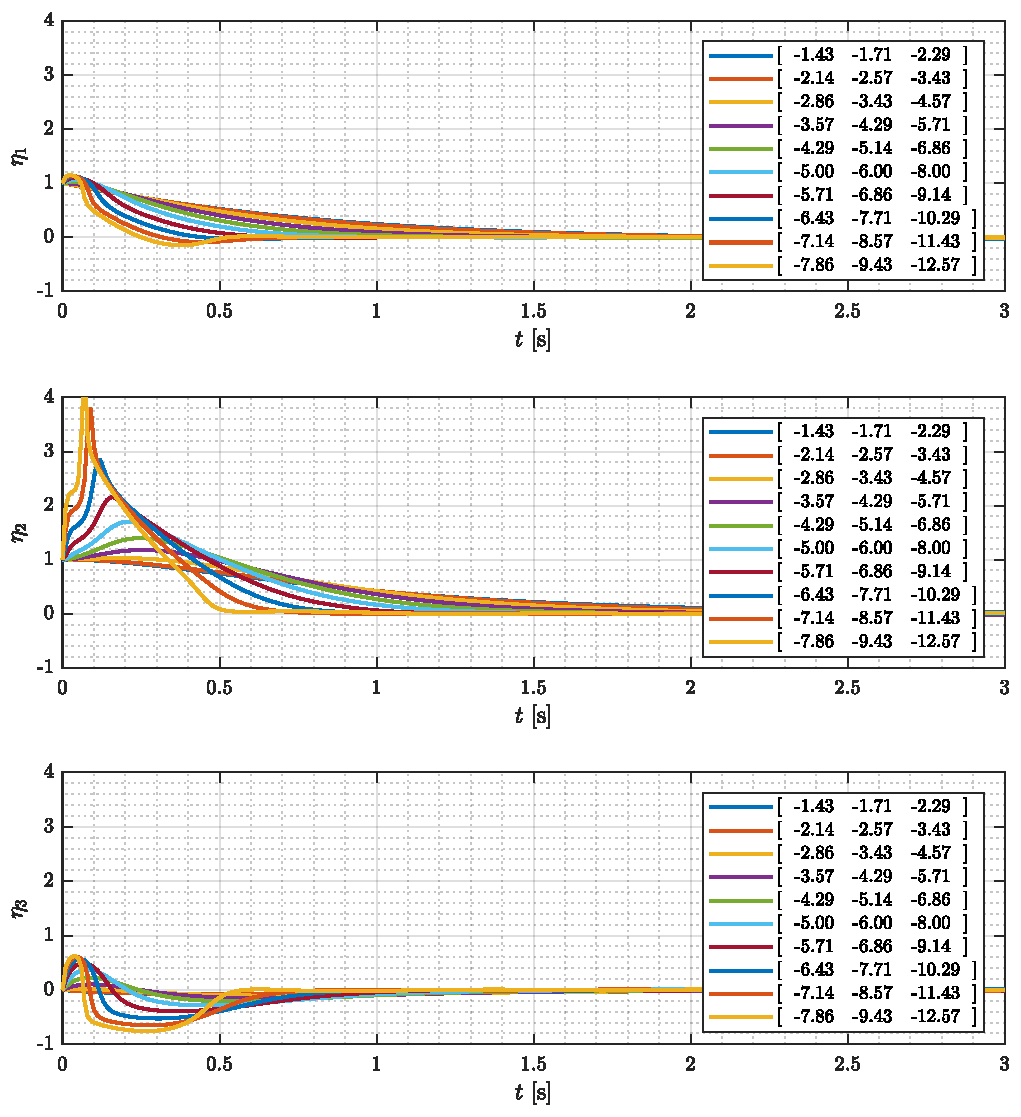
\includegraphics[width=\textwidth]{figures/reducedOrderControlMany}
    \end{figure}
  \end{minipage}
  \begin{minipage}{0.50\textwidth}
    \begin{figure}[H]
      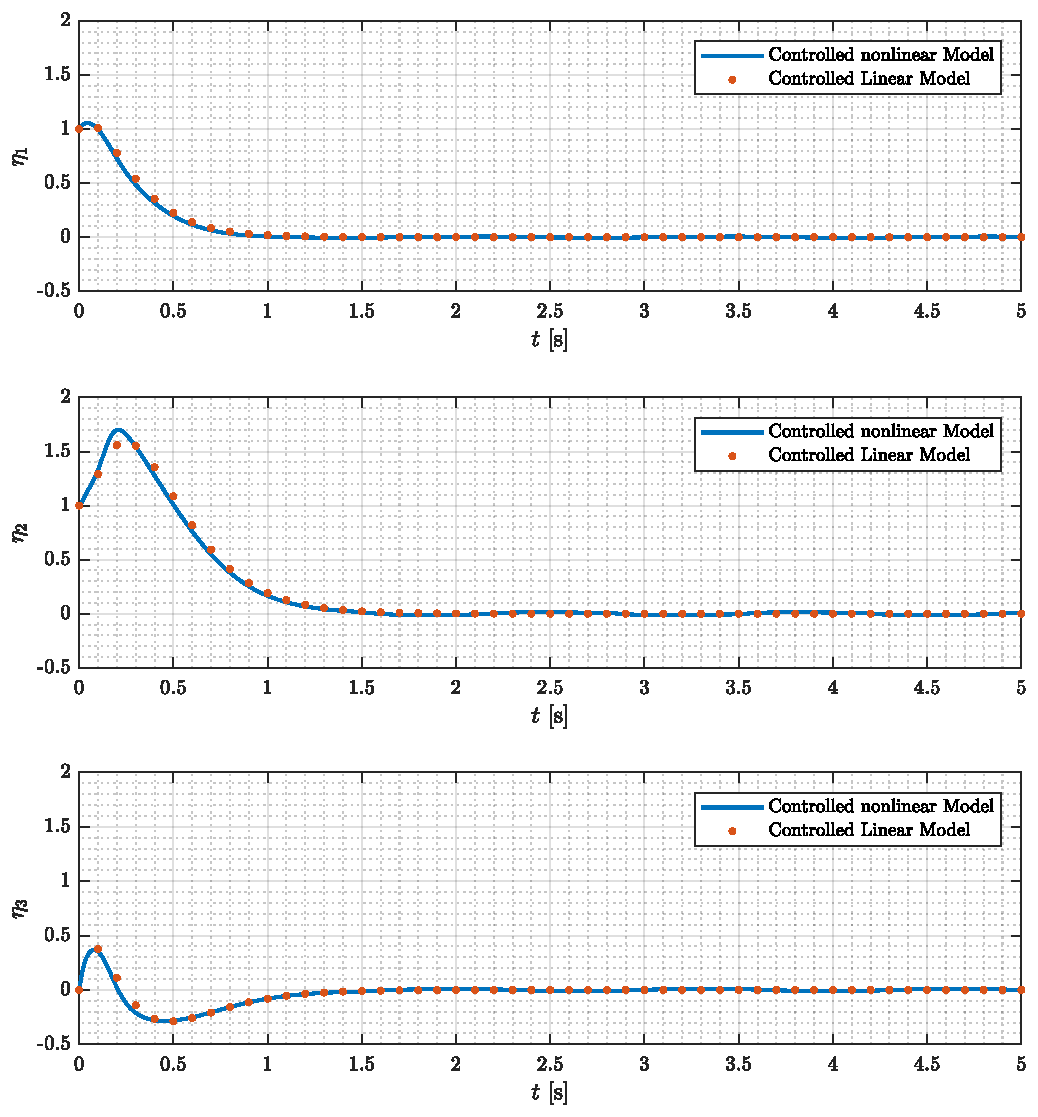
\includegraphics[width=\textwidth]{figures/reducedOrderControl}
    \end{figure}
  \end{minipage}
\end{minipage}
\end{frame}

\begin{frame}{Nonlinear Control}{Sliding Mode}
  \small
  %
  $V = \frac{1}{2}s^2$
  %
  \begin{flalign}
    \dot{V} &= s\dot{s} & \nonumber \\
    \dot{V} &= s ( \dot{\xi} + \vec{k}\dot{\vec{\eta}}  ) & \nonumber \\
    %\dot{V} &= s ( f_b(\vec{\eta},\xi) + g_b(\vec{\eta},\xi) F +\vec{k}f_a(\vec{\eta},\xi) )  & \nonumber \\
    %\dot{V} &= ( \vec{k}f_a(\vec{\eta},\xi)  +  f_b(\vec{\eta},\xi) )s + g_b(\vec{\eta},\xi) s F  & \nonumber \\
    \dot{V} &= g_b(\vec{\eta},\xi) s (\vec{k}f_a(\vec{\eta},\xi)  +  f_b(\vec{\eta},\xi)) g_b^{-1}(\vec{\eta},\xi) + g_b(\vec{\eta},\xi) s F  & \nonumber  \\
    \dot{V} &\leq g_b(\vec{\eta},\xi) |s| \left|\vec{k}f_a(\vec{\eta},\xi) g_b^{-1}(\vec{\eta},\xi) +  f_b(\vec{\eta},\xi) \right| + g_b(\vec{\eta},\xi) s F  \nonumber & \\
    \dot{V} &\leq g_b(\vec{\eta},\xi) |s| \left|\vec{k}f_a(\vec{\eta},\xi) +  f_b(\vec{\eta},\xi) \right|  g_b^{-1}(\vec{\eta},\xi)  & \nonumber \nonumber \\
    &- g_b(\vec{\eta},\xi) \text{sgn}(s) s \left|\vec{k}f_a(\vec{\eta},\xi)  +  f_b(\vec{\eta},\xi) \right| g_b^{-1}(\vec{\eta},\xi)  & \nonumber
  \end{flalign}
  \begin{flalign}
    F &= -\text{sgn}(s)\varrho(\vec{\eta},\xi) g_b^{-1}(\vec{\eta},\xi) \ \ \ \ \text{where}, \ \ \ \varrho(\vec{\eta},\xi)  \geq \left|\vec{k}f_a(\vec{\eta},\xi)  +  f_b(\vec{\eta},\xi) \right|  \nonumber &
  \end{flalign}
  %\begin{flalign}
  %F &= -\text{sgn}(s)\beta (\vec{\eta},\xi) g_b^{-1}(\vec{\eta},\xi) \ \ \ \ \text{where}, \ \ \ \beta(\vec{\eta},\xi) = \varrho(\vec{\eta},\xi) + \beta_0  & \nonumber
  %\normalsize
  %\end{flalign}
  \begin{flalign}
    F &= -\text{sat}(\tfrac{s}{\varepsilon})\beta (\vec{\eta},\xi)  g_b^{-1}(\vec{\eta},\xi) \ \ \ \ \text{where}, \ \ \ \beta(\vec{\eta},\xi) = \varrho(\vec{\eta},\xi) + \beta_0   & \nonumber
  \end{flalign}
  \normalsize
\end{frame}

\begin{frame}{Nonlinear Control}{Sliding Mode}
\small
  \begin{figure}[H]
    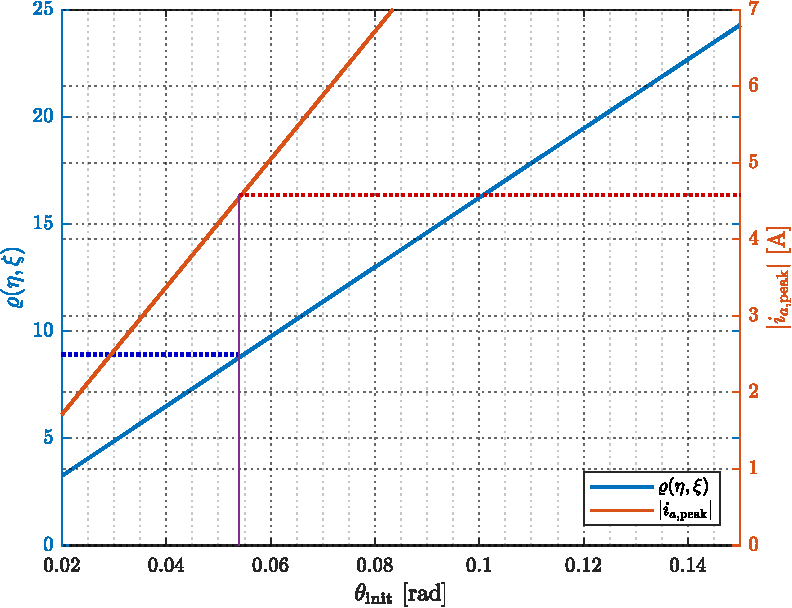
\includegraphics[width=.75\textwidth]{figures/chooseRho}
  \end{figure}
\normalsize
\end{frame}


%-------Nonlinear Control-----(Simulation)--------------------------------

\begin{frame}{Nonlinear Control}{Simulation}
  \hspace{-.9cm}
  \begin{minipage}{\textwidth}
    \begin{minipage}{0.56\textwidth}
      \begin{figure}[H]
        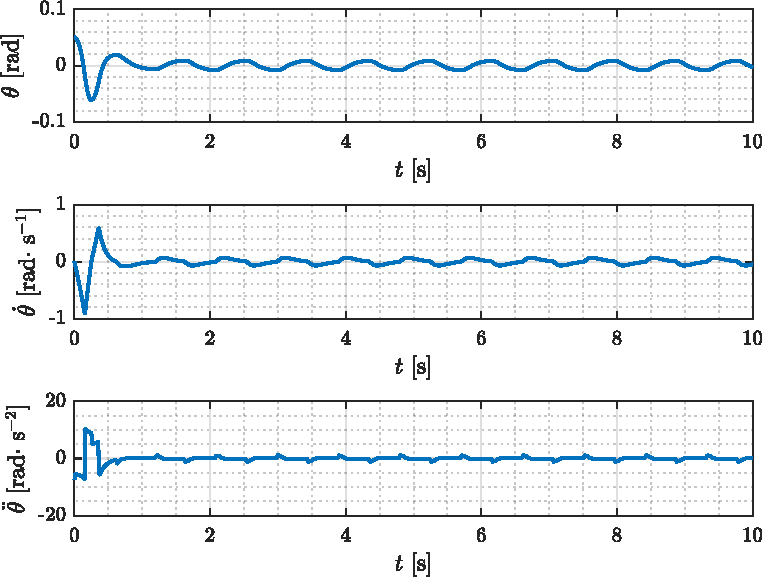
\includegraphics[width=\textwidth]{figures/slidingModeSIMtheta}
      \end{figure}
    \end{minipage}
    \begin{minipage}{0.56\textwidth}
      \begin{figure}[H]
        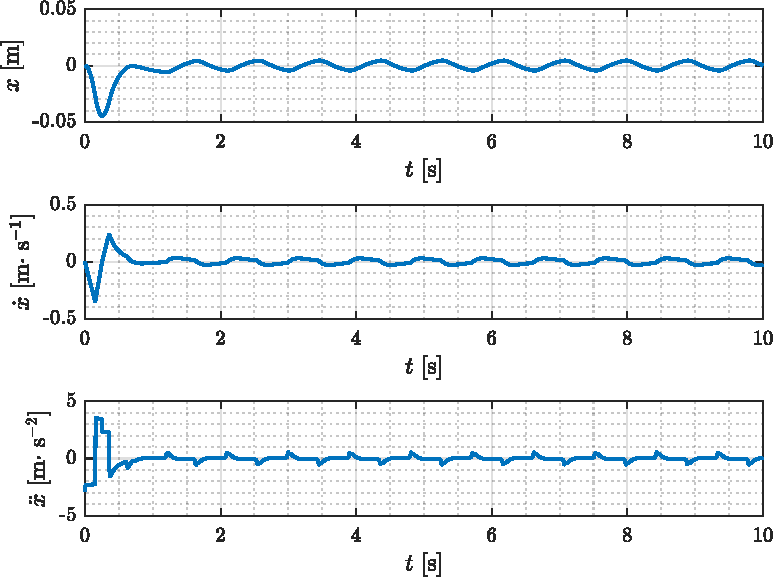
\includegraphics[width=\textwidth]{figures/slidingModeSIMx}
      \end{figure}
    \end{minipage}
  \end{minipage}
\end{frame}

\begin{frame}{Nonlinear Control}{Simulation}
\begin{figure}[H]
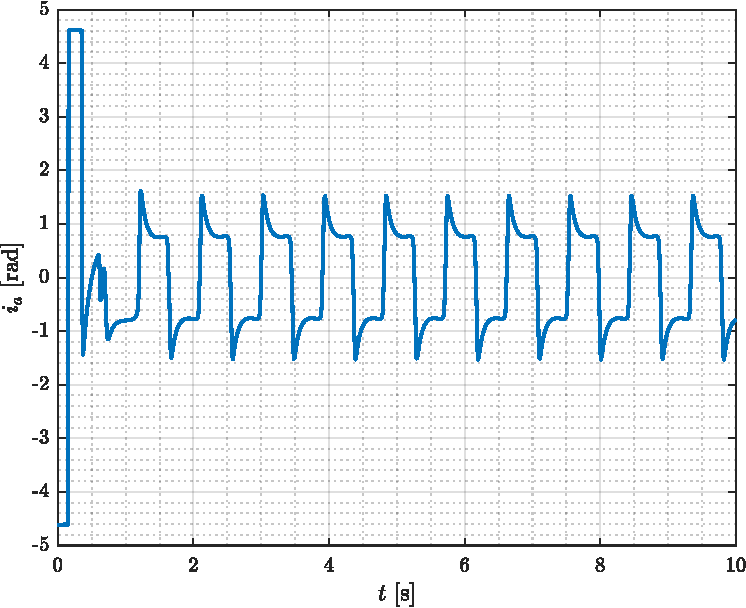
\includegraphics[width=.7\textwidth]{figures/slidingModeSIMia}
\end{figure}
\end{frame}


%-------Trajectory Planning--------------------------------------------------

\begin{frame}{Trajectory Planning}{System}
  \small
  \vspace{-.5cm}
  \begin{figure}[H]
    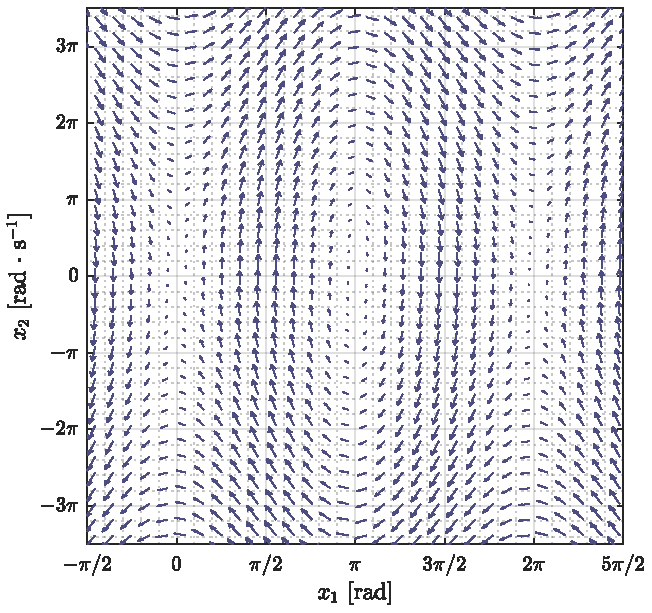
\includegraphics[width=.6\textwidth]{figures/modelPhasePlot}
  \end{figure}
  \vspace{-.5cm}
  \begin{flalign}
    \begin{cases}
    m l^2 \ddot{\theta} - m l \cos \theta \ddot{x} - m g l \sin \theta  = 0  & \nonumber \\   
    ( M + m )\ddot{x} + m l \sin \theta \dot{\theta}^2 - m l \cos \theta \ddot{\theta}  =  F   &  
    \end{cases} && \nonumber
  \end{flalign}
\normalsize
\end{frame}

\begin{frame}{Trajectory Planning}{Integral of System}
\small
  \vspace{-.5cm}
  \begin{flalign}
    \underbrace{ \left( m l^2 - \frac{m^2 l^2}{M + m} \cos^2 \theta \right)    }_{\alpha(\theta)}
    \ddot{\theta} +
    \underbrace{ \left( \frac{m^2 l^2}{M + m} \cos \theta \sin \theta \right)  }_{\beta(\theta)}
    \dot{\theta}^2
    \underbrace{ - m g l \sin \theta - \frac{m l}{M + m} \cos \theta F         }_{\gamma(\theta)}
    &=  0    && \nonumber
  \end{flalign}
  \begin{flalign}
  \alpha (\theta) \ddot{\theta} + \beta (\theta) \dot{\theta}^2 + \gamma (\theta) &=  0   \nonumber & 
  \end{flalign}
  %
  \begin{flalign}
  I(\theta,\dot{\theta},\theta_0,\dot{\theta}_0) &=
   \int \alpha (\theta) \ddot{\theta} + \beta (\theta) \dot{\theta}^2 + \gamma (\theta)\ d\theta   \nonumber &  
  \end{flalign}
  %
  \begin{flalign}
    I(\theta,\dot{\theta},\theta_0,\dot{\theta}_0) &=
    \dot{\theta}^2 -
    \text{exp}
    \left[ 
    -2 \int\limits_{\theta_0}^{\theta} \frac{\beta(\tau)}{\alpha(\tau)} d\tau
    \right]
    \left(
    \dot{\theta}_0^2 -
    \int\limits_{\theta_0}^{\theta}
    \text{exp}
    \left[
    2 \int\limits_{\theta_0}^{s} \frac{\beta(\tau)}{\alpha(\tau)} d\tau
    \right]
    \frac{2 \gamma (s)}{\alpha (s)}
    ds
    \right)  \nonumber &  
  \end{flalign}
\normalsize
\end{frame}

\begin{frame}{Trajectory Planning}{Trajectories}
  \small
  \vspace{-.25cm}
  \begin{flalign}
    I(\theta,\dot{\theta},\theta_0,\dot{\theta}_0) &=
    \dot{\theta}^2 -
    \text{exp}
    \left[ 
    -2 \int\limits_{\theta_0}^{\theta} \frac{\beta(\tau)}{\alpha(\tau)} d\tau
    \right]
    \left(
    \dot{\theta}_0^2 -
    \int\limits_{\theta_0}^{\theta}
    \text{exp}
    \left[
    2 \int\limits_{\theta_0}^{s} \frac{\beta(\tau)}{\alpha(\tau)} d\tau
    \right]
    \frac{2 \gamma (s)}{\alpha (s)}
    ds
    \right)  \nonumber &  
  \end{flalign}
  \begin{figure}[H]
    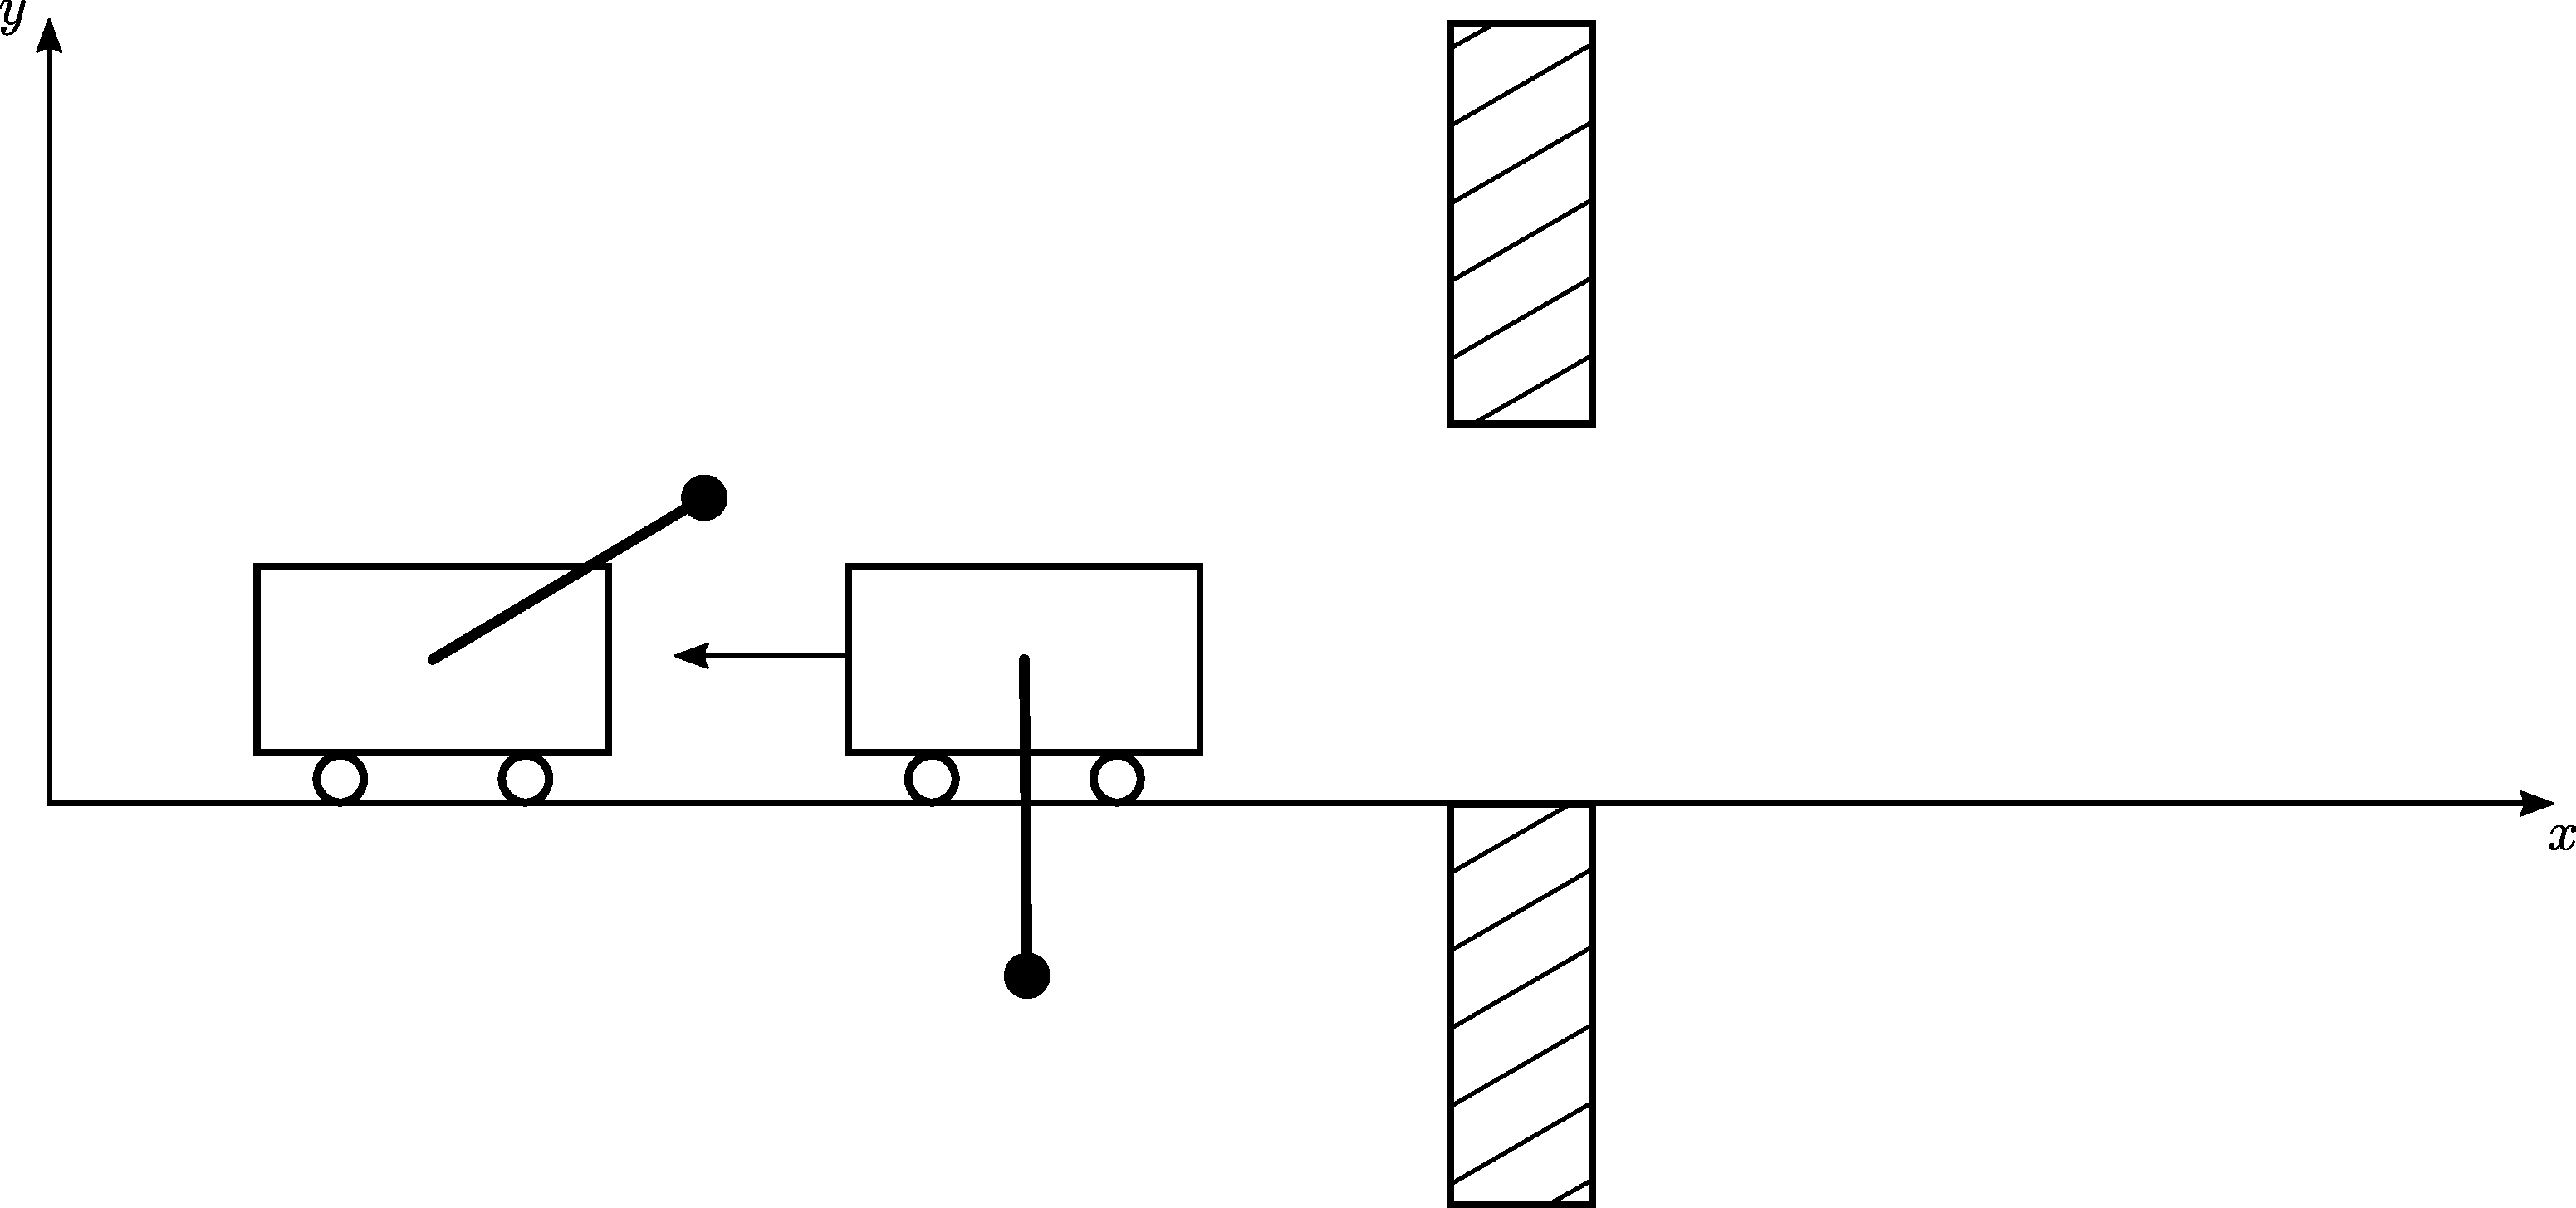
\includegraphics[width=.7\textwidth]{figures/firstTask}
  \end{figure}
  \begin{flalign}
    I(\theta,\dot{\theta},\theta_0,\dot{\theta}_0) &= \frac{m l^2 - \frac{m^2 l^2}{M + m}}{m l^2 - \frac{m^2 l^2}{M + m} \cos^2 \theta}
    \left(
    - 4 \left[ \frac{ M g + m g - F \tan\frac{s}{2} }{M l (\tan^2\frac{s}{2} + 1)}  \right]_{\theta_0}^\theta
    \right) & \nonumber
  \end{flalign}
  \normalsize
\end{frame}

\begin{frame}{Trajectory Planning}{Solution}
  \small
  \vspace{-.5cm}
  \begin{flalign}
    \begin{cases}
      m l^2 \ddot{\theta} - m l \cos \theta \ddot{x} - m g l \sin \theta  = 0  & \nonumber \\   
      ( M + m )\ddot{x} + m l \sin \theta \dot{\theta}^2 - m l \cos \theta \ddot{\theta}  =  F   &  
    \end{cases} && \nonumber
  \end{flalign}
  \begin{figure}[H]
    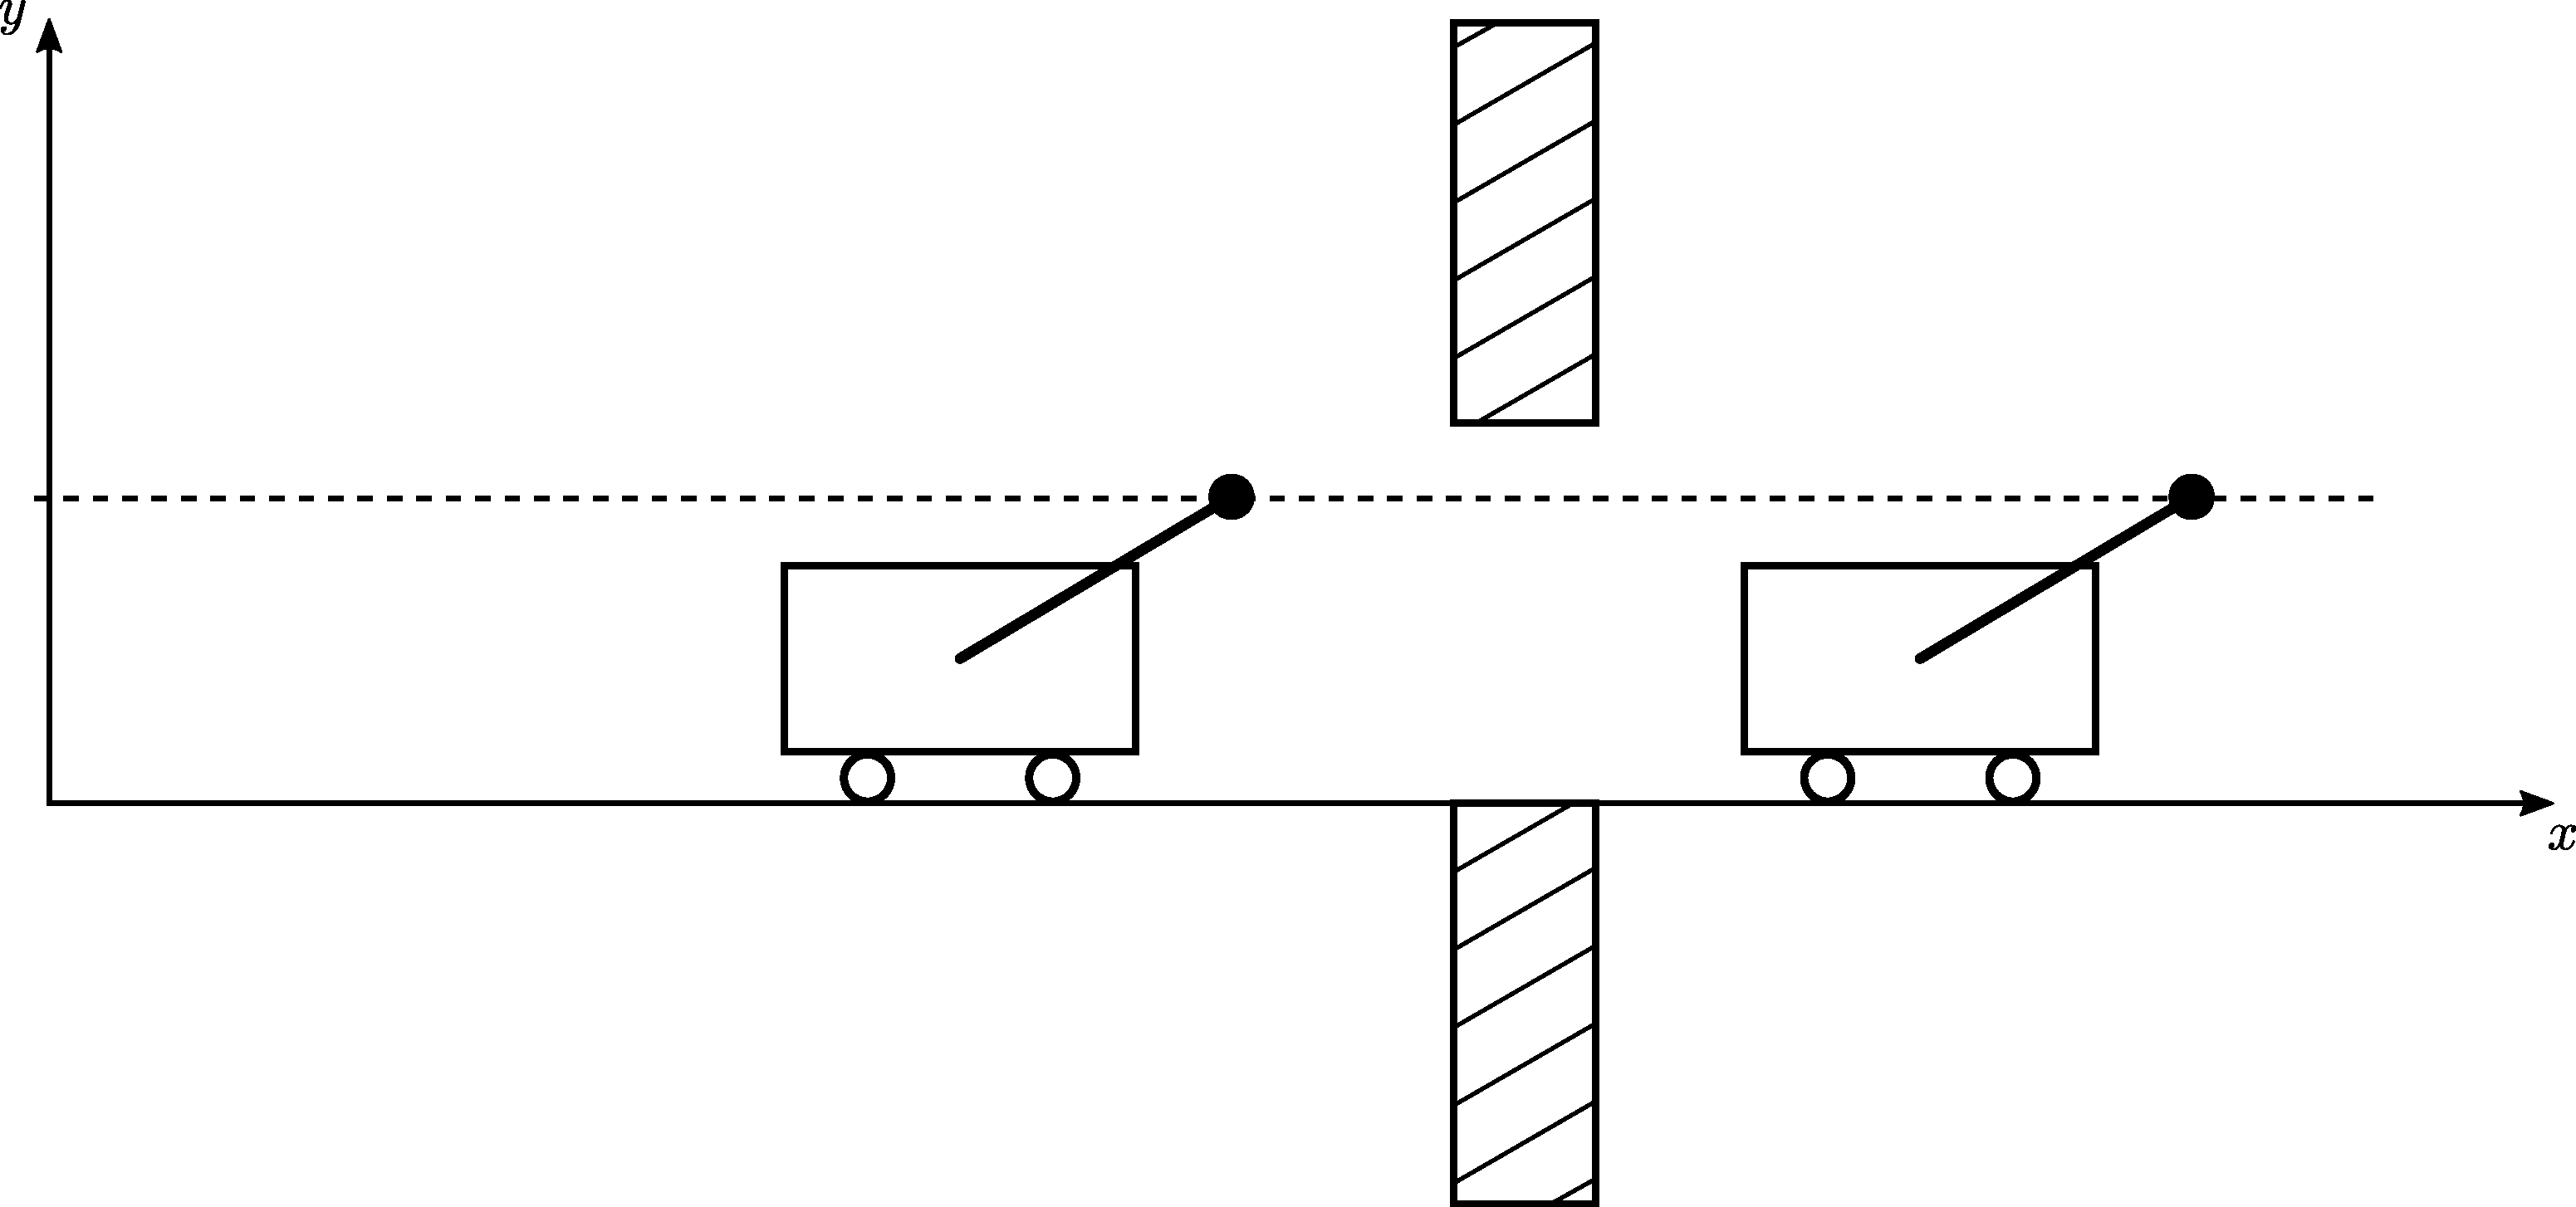
\includegraphics[width=.7\textwidth]{figures/secondTask}
  \end{figure}
  \vspace{-1cm}
  \begin{flalign}
  \begin{cases}
  - m l \cos \theta \ddot{x} - m g l \sin \theta  = 0  & \\
  ( M + m )\ddot{x}  =  F 
  \end{cases} \nonumber &&
  \end{flalign}
  \normalsize
\end{frame}


%-------Results-----(Sliding Mode)----------------------------------------

\begin{frame}{Results}{Sliding Mode}
\hspace{-.9cm}
\begin{minipage}{\textwidth}
  \begin{minipage}{0.56\textwidth}
    \begin{figure}[H]
      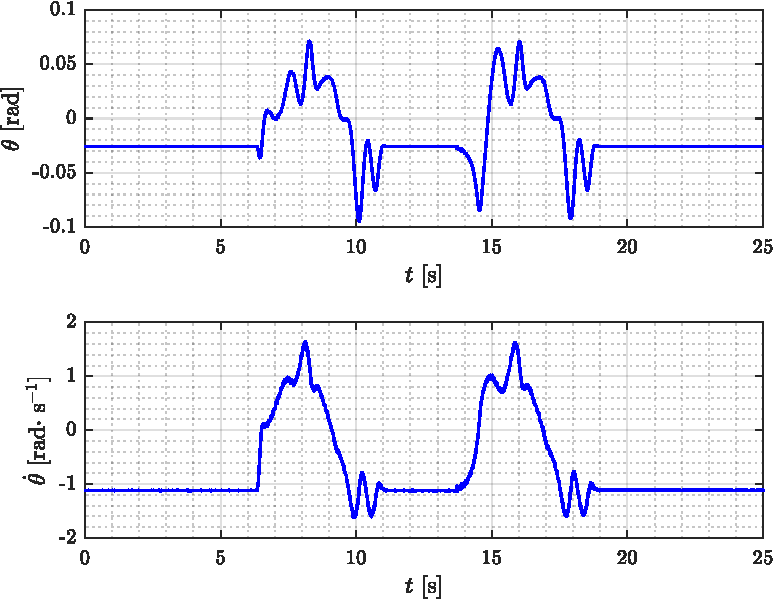
\includegraphics[width=\textwidth]{figures/slidingModeTest2theta}
    \end{figure}
  \end{minipage}
  \begin{minipage}{0.56\textwidth}
    \begin{figure}[H]
      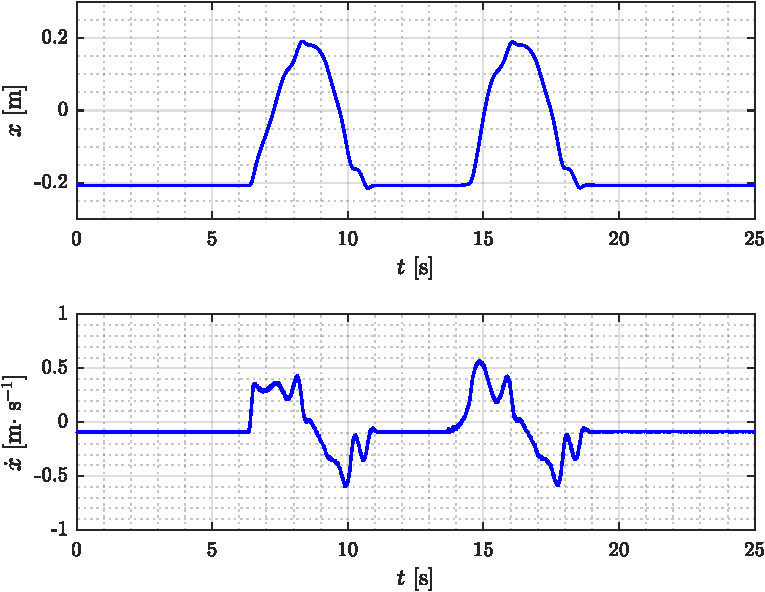
\includegraphics[width=\textwidth]{figures/slidingModeTest2x}
    \end{figure}
  \end{minipage}
\end{minipage}
\end{frame}

\begin{frame}{Results}{Sliding Mode}
\begin{figure}[H]
  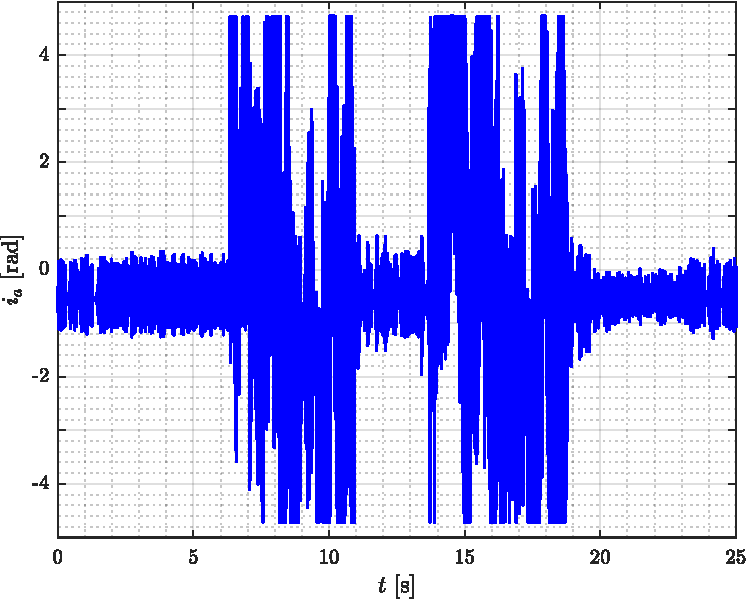
\includegraphics[width=.7\textwidth]{figures/slidingModeTest2ia}
\end{figure}
\end{frame}

%-------Results-----(Trajectory Planning)--------------------------------
  
\begin{frame}{Results}{Trajectory Planning}
\begin{figure}[H]
  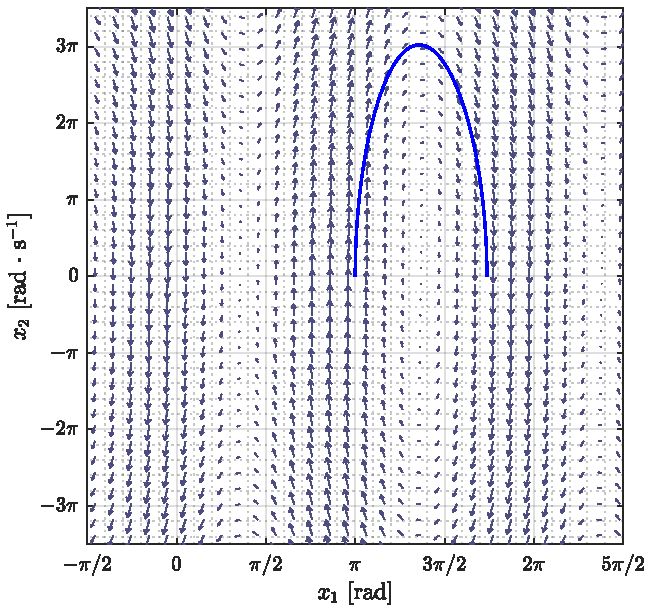
\includegraphics[width=.6\textwidth]{figures/firstTraj}
\end{figure}
\end{frame}

\begin{frame}{Results}{Trajectory Planning}
\begin{figure}[H]
  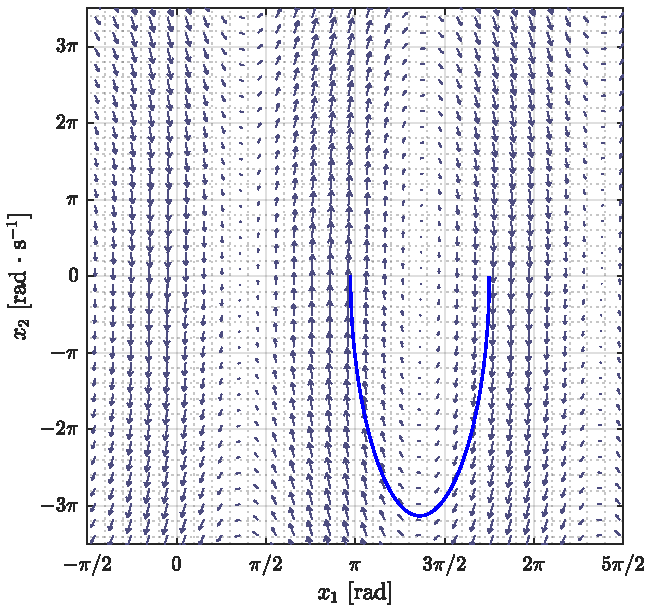
\includegraphics[width=.6\textwidth]{figures/thirdTraj}
\end{figure}
\end{frame}

\begin{frame}{Results}{Trajectory Planning}
\hspace{-1cm}
\begin{minipage}{1\textwidth}
  \begin{figure}[H]
    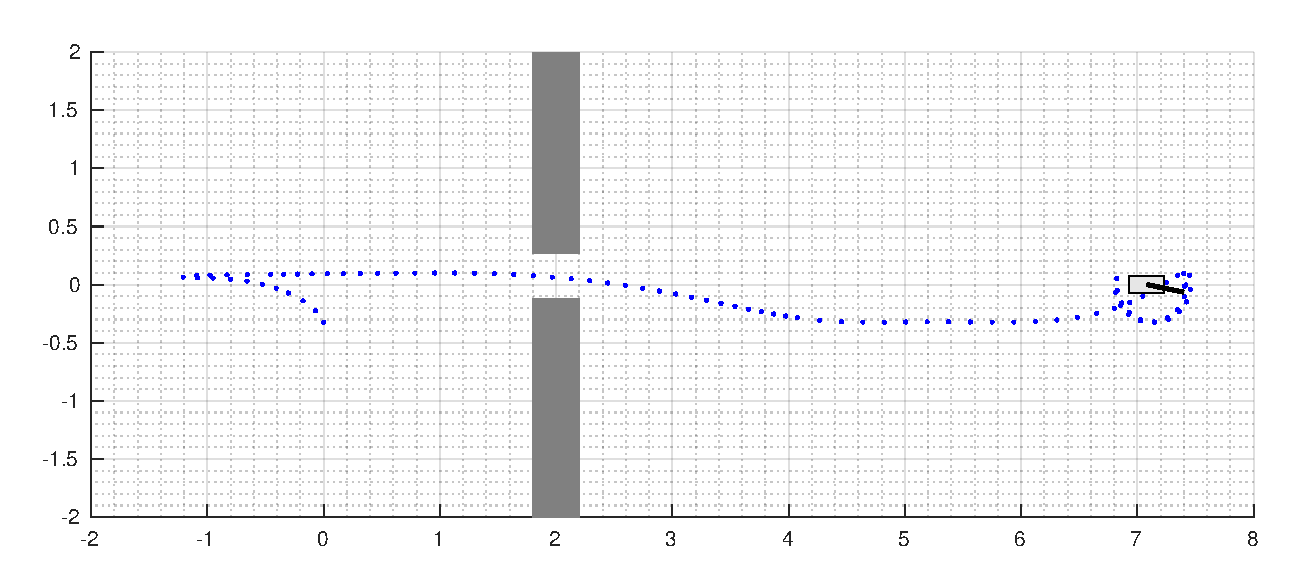
\includegraphics[width=1.15\textwidth]{figures/trajectoryAnimation}
  \end{figure}
\end{minipage}
\end{frame}